% ---------------------------------------------------------------------------
% PTEN missense variants in cBioPortal, ClinVar and gnomAD: cleaning,
% intersections, K-site profiles, and the ranking by the sampler's energies.
%
% Every number is measured and the log it comes from is named next to it. All
% logs and tables are in softmax/monte_carlo/pten_variants/; the code is
% softmax/monte_carlo/pten_variants.py (PRs #61 and the one carrying this file).
% Inputs: the three files in databases/ (commit cbce85c, 2026-11-18). No
% database or data host was contacted at any stage.
% Companion to pten_k_sites_explained.md (K-sets, scans) and pten_metrics.tex.
%
% Build:  cd softmax/docs && pdflatex pten_variants.tex && pdflatex pten_variants.tex
% ---------------------------------------------------------------------------
\documentclass[11pt,a4paper]{article}

\usepackage[T1]{fontenc}
\usepackage[utf8]{inputenc}
\usepackage[margin=2.3cm]{geometry}
\usepackage{amsmath,amssymb}
\usepackage{booktabs}
\usepackage{array}
\usepackage{graphicx}
\usepackage{float}
\usepackage{caption}
\usepackage{longtable}
\usepackage[hidelinks]{hyperref}
\newcolumntype{R}[1]{>{\raggedright\arraybackslash}p{#1}}
\sloppy
\captionsetup{font=small,labelfont=bf}

\newcommand{\file}[1]{\texttt{#1}}
\newcommand{\Uam}{U_{\mathrm{am}}}
\newcommand{\Uce}{U_{\mathrm{ce}}}
\newcommand{\Etwo}{E_{2}}

\title{PTEN missense variants in tumours, in patients and in the population:\\
three databases, the K-sites, and the sampler's energies}
\author{Marco Sanchini \\ \small\texttt{my\_extendedSampling} / \texttt{softmax}}
\date{2026--11--18}

\begin{document}
\maketitle

\begin{abstract}
\noindent
Three public collections of PTEN missense variants were cleaned, deduplicated
and intersected: somatic mutations in tumours (cBioPortal, TCGA PanCancer
Atlas), germline submissions (ClinVar) and population alleles (gnomAD). After
cleaning they hold 1269 distinct changes on canonical PTEN, 1093 of them inside
the 324-residue construct the sampler uses. Two questions were asked of them.
\emph{Where do the variants land?} Variants from tumours and ClinVar
pathogenic variants are 3.6--4.3 times more frequent than chance at the sites
conserved across the PTEN family, 2.6--2.8 times at the sites where yeast
activity is lost, 2.2--3.3 times at the sites the sampler itself keeps
conserved, and only 1.3--1.4 times at the sites that control abundance;
population variants are spread uniformly. \emph{Do the sampler's energies
recognise them?} The attention-map energy $\Uam$ separates disease from
population variants with AUC 0.67--0.70, the structure-token cross-entropy
$\Uce$ with 0.70--0.77, while the two-step contact-map energy $\Etwo$ of Zambon
et al.\ is at chance (0.49--0.54). $\Uam$ carries its information in the
substitution, $\Uce$ in the site. The most frequent tumour mutations, at
R130, are stable and catalytically dead, and every energy that reads the fold
ranks them as unremarkable. Compound tumour sequences carrying 2--5 PTEN
mutations are close to additive in $\Uam$ (median ratio 0.93), sub-additive in
$\Uce$ (0.77) and saturated in $\Etwo$ (0.49).
\end{abstract}

\tableofcontents

% ===========================================================================
\section{Premises}
% ===========================================================================

\subsection{The question}

The thesis studies the sequence landscape of an effective energy that ESM3
defines around a reference protein, and the sampler that explores it. For PTEN
(reference \file{pten\_1d5r}) two independent benchmarks have been used so far:
natural sequence variation across species, and two deep mutational scans
(VAMP-seq abundance, Matreyek et al.\ 2018/2021; yeast lipid-phosphatase
activity, Mighell et al.\ 2018). This note adds a third: variation observed in
\emph{humans}, in three forms.
\begin{itemize}
\item \textbf{Tumours} (cBioPortal): somatic mutations; recurrent ones are
  likely drivers, i.e.\ they destroy PTEN's tumour-suppressor function.
\item \textbf{Patients} (ClinVar): germline variants submitted by diagnostic
  laboratories and classified as pathogenic, uncertain or benign, mostly for
  PTEN hamartoma tumour syndrome (PHTS).
\item \textbf{Population} (gnomAD): alleles seen in hundreds of thousands of
  people without selection for disease; as a class, tolerated.
\end{itemize}
Human population variation is something the natural alignments cannot show:
UniRef90 clusters at 90\% identity, so within-species variation never enters
them (\file{pten\_k\_sites\_explained.md}).

The request was: analyse each database separately and all three merged; check
duplicates within and intersections between them; build K-site entropy
profiles for categories of variants; and rank the variants by $\Uam$ and by
Zambon's contact-map energy at two decoding steps.

\subsection{Data, and what was not done}

The three files were pushed to \file{databases/} on 2026-11-18 (commit
\texttt{cbce85c}): \file{cbioportal\_pten.tsv}, \file{clinvar\_download\_%
20261118\_064848.tsv}, \file{gnomAD\_download\_pten.csv}. \textbf{No database
or data host was contacted}: every number below comes from these files and
from tables already in the repository or on astaroth. The single external
table used is \file{PTEN\_variant\_data.tsv} (FowlerLab VAMP-seq release),
already on astaroth since PR\,\#45, for its genetic-code column.

\subsection{Numbering}

Canonical PTEN: UniProt P60484, RefSeq NM\_000314, Ensembl ENST00000371953,
403 residues. The construct \file{pten\_1d5r} is UniProt 7--285 and 310--353
(the 286--309 loop deleted, as in crystal 1D5R), 324 sites; sites 0 and 279
are not native. Domains: N-terminus 1--13, phosphatase 14--185, C2 186--351,
C-tail 352--403.

\subsection{The three energies}

All three were already computed for the 324$\times$19 = 6156 single mutants of
the construct; this note only looks them up.

\begin{description}
\item[$\Uam$] The sampler's energy,
  $\Uam = \sum_{i<j}\left[\log A_{ij}(s) - \log A_{ij}(\mathrm{ref})\right]^2$
  over ESM3's symmetrised final-layer attention map. $\Uam(\mathrm{ref})=0$ is
  the global minimum, so for a single mutant $\Delta U = \Uam$. Scan
  \file{pten\_single\_mutants.csv}, \texttt{--batch 1}, bit-reproducible
  (PR\,\#49).
\item[$\Etwo$] Zambon et al.\ (2024)'s normalised contact-map difference,
  $E = \sum_{ij}|D_{ij}(s)-D_{ij}(\mathrm{ref})| / \sum_{ij}(D_{ij}(s)+D_{ij}(\mathrm{ref}))$,
  $|i-j|>2$, on the C$_\alpha$ map at 8\,\AA, both maps decoded by ESM3 at two
  generation steps. Scan \file{pten\_mutants\_E2.csv}. Known from 2026-11-17:
  per mutant, $E$ depends on the number of decoding steps (Spearman between 4
  and 32 steps $-0.002$); per site it is stable.
\item[$\Uce$] The cross-entropy of the predicted structure tokens against
  the reference's own, minus its reference value: the second, so far unused,
  term of the sampler's energy. Scan \file{pten\_mutants\_ce.csv}, float32
  (PR\,\#60).
\end{description}
For all three, \emph{higher = more costly = predicted damaging}.

\subsection{The K-sets}

``K-sites'' are the sites the sampler keeps conserved (Zambon 2024), compared
with three external definitions of ``this site cannot change''
(\file{pten\_k\_sites.py}, PR\,\#45/\#47):
\begin{description}
\item[K\_natural] (28 sites) entropy $<0.5$ nats in the PTEN-like family
  alignment (2716 sequences, 59\% tensins).
\item[K\_abundance] (108) sites where VAMP-seq abundance collapses: the fold.
\item[K\_activity] (97) sites where yeast activity is lost: largely catalysis.
\item[K\_sampled\_T4, K\_sampled\_T8] (33 each) new here: the 10\% of native
  sites with the lowest sampled entropy at $T=4$ and $T=8$. Entropy from the
  \file{equil\_ref} chains 0 and 1 (400\,001 moves at $T=4$, 150\,001 at
  $T=8$), averaged, with \texttt{--burn-in-frac 0.8}, which clears $t_{\mathrm{eq}}$
  at every temperature. The cut-offs are 0.168 and 0.677 nats. A fixed
  threshold near zero would leave a handful of sites at these temperatures.
\end{description}

\subsection{The genetic-code confound}

A missense variant observed in a person almost always differs from the
reference codon by a single base: of the 19 substitutions at a site only 2--9
are reachable that way. The earlier look at COSMIC counts
(\file{pten\_k\_sites\_explained.md} 10.5) showed that without this control
the AUC of $\Uam$ against ``observed in tumours'' is 0.51, i.e.\ nothing,
because the scan enumerates all 19 substitutions and the observed ones are a
biased subset. Every density and every enrichment below is therefore computed
over SNV-reachable substitutions only, and every AUC is reported on them.

% ===========================================================================
\section{Cleaning and deduplication}
% ===========================================================================

Every variant is reduced to a protein key \texttt{wt+position+mut} on
canonical PTEN, and every wild-type letter is checked against the canonical
sequence (0 mismatches in all three files). A DNA key (GRCh38
\texttt{chr:pos:ref:alt}) is kept alongside. Log: \file{clean.log}.

\subsection{Three traps in the raw files}

\begin{enumerate}
\item \textbf{ClinVar's header is one field short.} The header has 24
  tab-separated fields, every data row 25. A plain \texttt{read\_csv} then uses
  the first column as the row index and shifts every label one place: the
  column called ``Molecular consequence'' holds the classification. The script
  counts the fields, reads with \texttt{index\_col=False}, and refuses to go on
  if ``Variant type'' does not contain ``single nucleotide variant''.
\item \textbf{PTEN-L.} An upstream, non-AUG start adds 173 residues
  (PTEN-Long). ClinVar lists both numberings in its ``Protein change'' column
  (\texttt{M174L, M1L}); gnomAD puts 232 of its 469 missense rows on
  ENST00000693560, whose extra exon is the 5$'$ UTR of canonical PTEN. Those
  rows include ``C65S, allele frequency 0.994'' and ``G4R, 0.143'', which are
  not residues 65 and 4 of PTEN. Only the \texttt{NM\_000314(PTEN)} HGVS in
  ClinVar's ``Name'' and only ENST00000371953 rows in gnomAD are used.
\item \textbf{KLLN} shares PTEN's promoter. Five ClinVar missense rows are
  named on KLLN; two gnomAD rows (S153 on ENST00000472832) are intronic in
  PTEN. They go with the same filter.
\end{enumerate}

\subsection{Rules per database}

\begin{table}[H]
\centering\small
\begin{tabular}{@{}R{2.2cm}R{4.6cm}R{4.6cm}r@{}}
\toprule
Database & What was found & Rule & Changes kept \\
\midrule
cBioPortal & 1203 rows, 25 TCGA studies; 516 missense rows in 418 samples / 417
patients. No (sample, change) duplicate. One patient with the same change in
two samples. 77 samples with 2--5 PTEN missense. 6 protein changes from two
different DNA changes (C124S, D92E, G129R, G36R, S10R, W111R). 119 samples
with $>500$ mutations carry 179 rows. &
One count per patient. Multi-mutation samples kept as compound sequences
(section~\ref{sec:compound}). Hypermutated samples flagged, every tumour
result also given without them. & 263 \\[2pt]
ClinVar & 4277 variations; 1355 with a missense consequence; 1223 canonical
missense rows. No duplicate VariationID or SPDI. 55 protein changes carried by
2+ variations (other codons; 22 MNV/indel rows). Classes: 798 VUS, 274 P/LP,
141 conflicting, 10 B/LB. &
One row per protein change; class = most severe call among the rows with the
highest review status (expert panel $>$ multiple submitters $>$ single).
Conditions grouped into PHTS, autism/macrocephaly, cancer. & 1164 \\[2pt]
gnomAD & 1868 alleles, 469 missense, 235 on the canonical transcript. No
duplicate; all pass the joint filter; 42 in segdup/lcr regions (flagged,
kept). 146 singletons, 89 with AC $\ge 2$, one site with a homozygote. &
Canonical transcript only; allele counts summed per protein change. & 235 \\
\bottomrule
\end{tabular}
\caption{What each file holds and the rule applied. ClinVar has only 10
benign/likely benign missense variants, so ClinVar cannot supply the tolerated
class; gnomAD does.}
\end{table}

\subsection{SNV reachability from the files' own codons}

Every single-nucleotide change written \texttt{c.N X>Y} on the canonical
transcript (missense, synonymous and nonsense alike) names the reference base
at CDS position $N$. The three files name 1065 of the 1212 CDS bases; with the
protein sequence constraining the rest, 362 of 403 codons resolve to a single
codon. A substitution is SNV-reachable when it is one base away from every
candidate codon. On astaroth the \texttt{snv} column of
\file{PTEN\_variant\_data.tsv} \textbf{agrees with this reconstruction on all
7532 substitutions both define} and fills the remainder: 2397 of 7657
substitutions are reachable, 5260 are not, 0 are unknown. Inside the construct
1906 of 6156 are reachable, the same number the COSMIC look found
independently. Check built into \file{clean}: all 1951 variants observed as
SNVs come out reachable. The 12 observed but unreachable changes are ClinVar
multi-nucleotide variants.

% ===========================================================================
\section{Intersections}
% ===========================================================================

\begin{table}[H]
\centering\small
\begin{tabular}{@{}lrr@{}}
\toprule
Set (exclusive regions) & Variants & In construct \\
\midrule
cBioPortal only & 64 & 60 \\
ClinVar only & 796 & 687 \\
gnomAD only & 38 & 30 \\
cBioPortal + ClinVar & 174 & 170 \\
cBioPortal + gnomAD & 3 & 2 \\
ClinVar + gnomAD & 172 & 122 \\
all three & 22 & 22 \\
\midrule
union & 1269 & 1093 \\
\bottomrule
\end{tabular}
\caption{Overlaps on the protein key (\file{merge.log}). Outside the
construct: 93 in the C-tail, 60 in the 286--309 loop, 23 in the N-terminus.}
\end{table}

\paragraph{DNA level.} cBioPortal is on GRCh37, gnomAD on GRCh38, ClinVar on
both. Over the PTEN locus GRCh37 $-$ GRCh38 $= 1\,759\,757$ for all 3000
ClinVar SNVs that carry both coordinates, so cBioPortal is lifted by that
constant (re-checked on every run; the script stops if it fails). On the DNA
key: C$\cap$V 196, C$\cap$G 23, V$\cap$G 189, all three 20. Four protein
changes are shared by cBioPortal and ClinVar through a different codon change.

\paragraph{What the overlaps say.}
\begin{itemize}
\item gnomAD sits largely inside ClinVar (194 of 235): laboratories submit the
  rare variants they meet, and ClinVar files most of them as VUS.
\item 25 tumour changes are also in gnomAD, among them the hotspots R173C (13
  patients, gnomAD AC 5), R142W (11, AC 5), R130L (7, AC 1) and P246L (6, AC
  3). 24 ClinVar P/LP changes are in gnomAD, all at AC $\le 5$. For a
  tumour suppressor with a dominant syndrome, ``seen in gnomAD'' is not
  ``benign''; the population categories below exclude P/LP where it matters.
\end{itemize}

\paragraph{Cross-references.} cBioPortal's own ClinVar column labels 184 of
the variants; 19 disagree with the ClinVar file (an older snapshot, mostly VUS
$\leftrightarrow$ conflicting). gnomAD's labels 189; one disagrees (F241L,
conflicting in gnomAD, P/LP in the file). The ClinVar file is used throughout;
the list is in \file{merge.log}.

\begin{figure}[H]
\centering
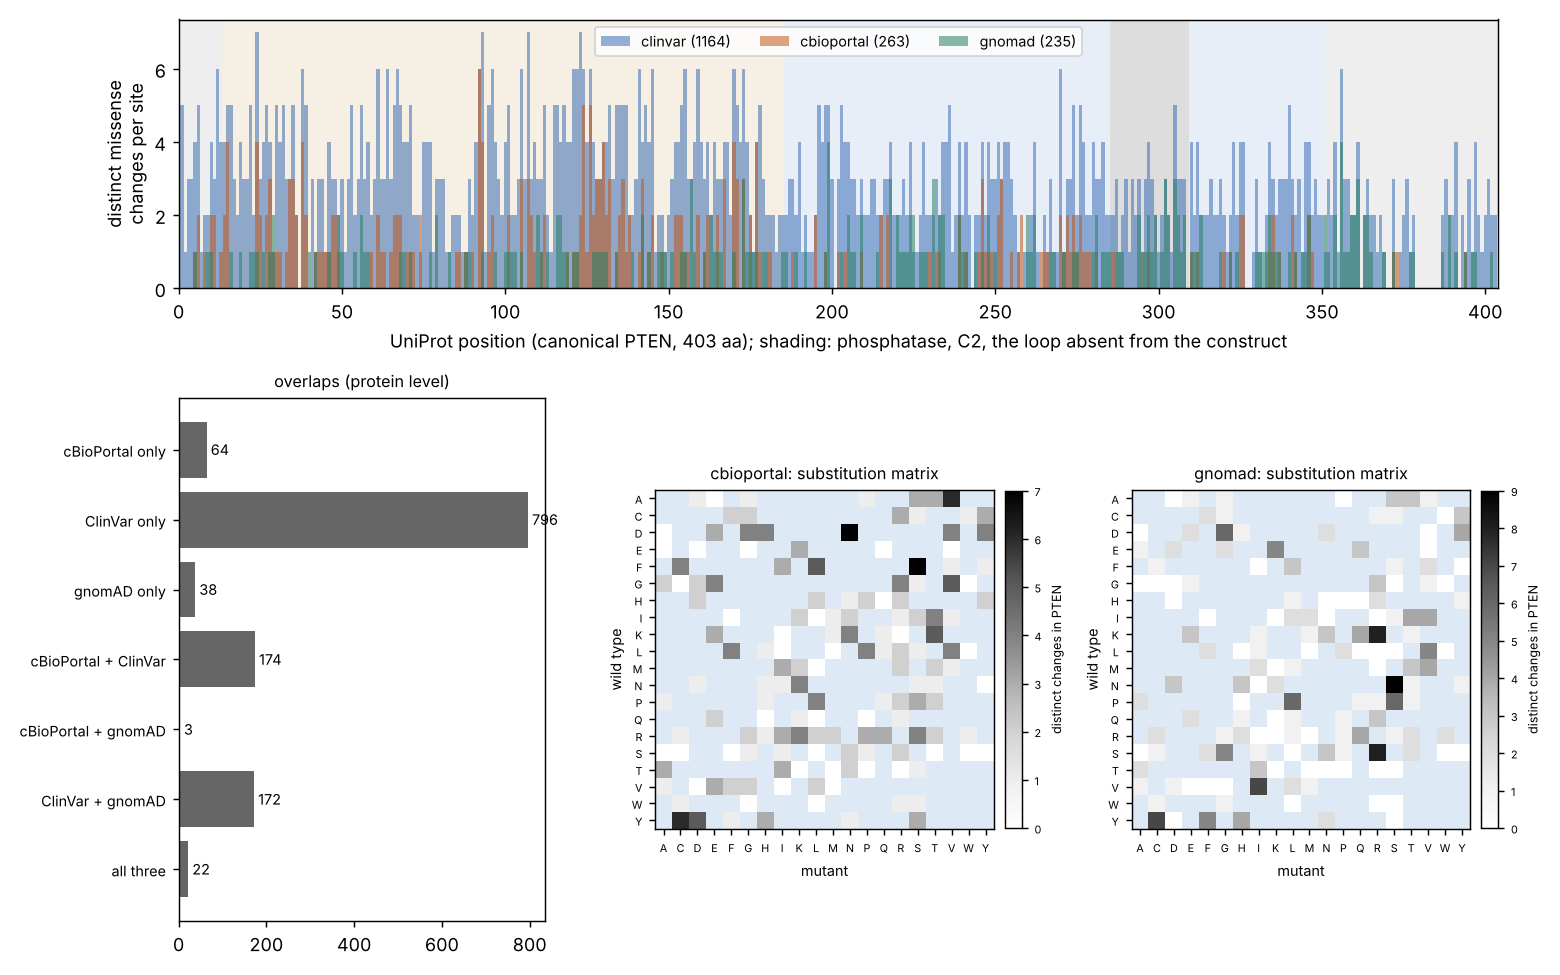
\includegraphics[width=\linewidth]{figures/pten_var_overview.png}
\caption{Top: distinct missense changes per position, per database, along
canonical PTEN (shading: N-terminus, phosphatase, C2, the 286--309 loop absent
from the construct, C-tail). Bottom: the overlaps, and the substitution
matrices of tumour and population variants.}
\end{figure}

% ===========================================================================
\section{Categories}
% ===========================================================================

\begin{table}[H]
\centering\small
\begin{tabular}{@{}llR{5.0cm}r@{}}
\toprule
Group & Category & Definition & $n$ \\
\midrule
cBioPortal & all & in any tumour & 254 \\
 & recurrent & in 2+ patients & 73 \\
 & singleton & in 1 patient & 181 \\
 & non-hypermutated & in 1+ patient with $\le 500$ mutations & 194 \\
 & endometrial / glioblastoma & in that cancer type & 128 / 58 \\
 & second hit & with ShallowDel/DeepDel of the other allele & 124 \\
ClinVar & all / P/LP / VUS / conflicting & collapsed class & 989 / 247 / 624 / 114 \\
 & expert & review status $\ge$ expert panel & 117 \\
 & PHTS / autism & condition group & 691 / 38 \\
gnomAD & all / singleton / AC$\ge$2 & & 176 / 121 / 55 \\
merged & all & in any database & 1081 \\
 & tumour-only & tumour, not gnomAD & 230 \\
 & population-only & gnomAD, not tumour & 152 \\
 & tumour and population & both & 24 \\
 & consensus damaging & ClinVar P/LP or tumour-recurrent, and not tolerated & 275 \\
 & consensus tolerated & gnomAD AC$\ge$2, not P/LP, not damaging & 47 \\
\bottomrule
\end{tabular}
\caption{The categories, with $n$ = distinct SNV-reachable variants inside the
construct (the number every K-set test uses). Categories with fewer than 20
variants would be reported as counts only; none fell below.}
\label{tab:cats}
\end{table}

% ===========================================================================
\section{K-site profiles}
% ===========================================================================

\subsection{Method}

For each category and construct site $i$ (\file{profiles.log},
\file{kset\_profiles.tsv}):
\begin{itemize}
\item \textbf{density} $\rho_i$ = observed SNV-reachable changes at $i$ /
  SNV-reachable changes at $i$;
\item \textbf{substitution entropy} $H_i = -\sum_a p_a\log p_a$ (nats) of the
  observed mutant residues at $i$, weighted by patients (cBioPortal), allele
  count (gnomAD) or one per variation (ClinVar); same units as the sampled and
  natural entropies.
\end{itemize}
Enrichment in a K-set: the number of the category's variants inside the set
against a uniform draw over the 1906 SNV-reachable substitutions of the
construct, so that a site with more reachable substitutions expects more
variants; two-sided binomial $p$. A second $p$ comes from circular shifts of
the set along the sequence (keeps the run structure of neighbouring sites;
smallest value $1/324 = 0.0031$). Correlations: Spearman of $\rho_i$ with each
per-site reference, raw and with the relative solvent accessibility (RSA) of
1D5R regressed out.

\subsection{Enrichment}

\begin{table}[H]
\centering\small
\begin{tabular}{@{}lrrrrr@{}}
\toprule
Category & natural & abundance & activity & sampled T4 & sampled T8 \\
\midrule
tumour, all & 2.90 & 1.45 & 2.24 & 2.06 & 1.91 \\
tumour, recurrent & \textbf{4.32} & 1.31 & 2.81 & 3.16 & 3.32 \\
tumour, singleton & 2.33 & 1.50 & 2.01 & 1.62 & 1.34 \\
tumour, non-hypermutated & 3.19 & 1.52 & 2.50 & 2.00 & 2.08 \\
tumour, endometrial & 3.38 & 1.31 & 2.31 & 2.45 & 2.28 \\
tumour, glioblastoma & 3.02 & 1.44 & 2.43 & 2.53 & 2.43 \\
tumour, second hit & 3.87 & 1.33 & 2.52 & 2.53 & 2.20 \\
ClinVar, all & 1.45 & 1.14 & 1.35 & 1.18 & 1.28 \\
ClinVar P/LP & 3.69 & 1.38 & 2.67 & 2.16 & 2.61 \\
ClinVar VUS & 0.52 & 1.01 & 0.74 & 0.77 & 0.73 \\
ClinVar conflicting & 1.74 & 1.39 & 1.80 & 1.29 & 1.50 \\
ClinVar expert panel & 3.40 & 1.28 & 2.24 & 2.51 & 2.41 \\
ClinVar PHTS & 1.62 & 1.16 & 1.48 & 1.29 & 1.36 \\
ClinVar autism/macrocephaly & 1.23 & 1.42 & 1.59 & 1.10 & 1.33 \\
gnomAD, all & 0.93 & 0.87 & 0.82 & 0.83 & 0.86 \\
gnomAD, singleton & 0.97 & 0.96 & 0.94 & 0.95 & 0.75 \\
gnomAD, AC$\ge$2 & 0.85 & 0.65 & 0.55 & 0.57 & 1.10 \\
merged, all & 1.40 & 1.14 & 1.32 & 1.15 & 1.20 \\
tumour-only & 2.80 & 1.45 & 2.22 & 2.05 & 1.80 \\
population-only & 0.46 & 0.79 & 0.58 & 0.62 & 0.53 \\
tumour and population & 3.90 & 1.37 & 2.38 & 2.18 & 2.94 \\
consensus damaging & 3.61 & 1.39 & 2.62 & 2.17 & 2.60 \\
consensus tolerated & \textbf{0.25} & 0.51 & 0.21 & 0.67 & 0.86 \\
\bottomrule
\end{tabular}
\caption{Variants inside each K-set, observed / expected
(\file{kset\_enrichment.tsv}). Selected two-sided binomial $p$: consensus
damaging $7\times10^{-26}$, $1\times10^{-5}$, $2\times10^{-60}$,
$4\times10^{-8}$, $8\times10^{-14}$; tumour recurrent $4\times10^{-11}$,
$0.08$, $4\times10^{-21}$, $1\times10^{-6}$, $1\times10^{-7}$; ClinVar P/LP
$1\times10^{-24}$, $5\times10^{-5}$, $6\times10^{-58}$, $2\times10^{-7}$,
$1\times10^{-12}$; gnomAD all $0.9$, $0.2$, $0.1$, $0.6$, $0.6$; autism $0.8$,
$0.1$, $0.03$, $1.0$, $0.6$. The circular-shift $p$ is at most 0.015 for every enrichment above 2,
and at its floor (0.0031) for all of them except the 24 tumour-and-population
variants.}
\label{tab:enrich}
\end{table}

\begin{figure}[H]
\centering
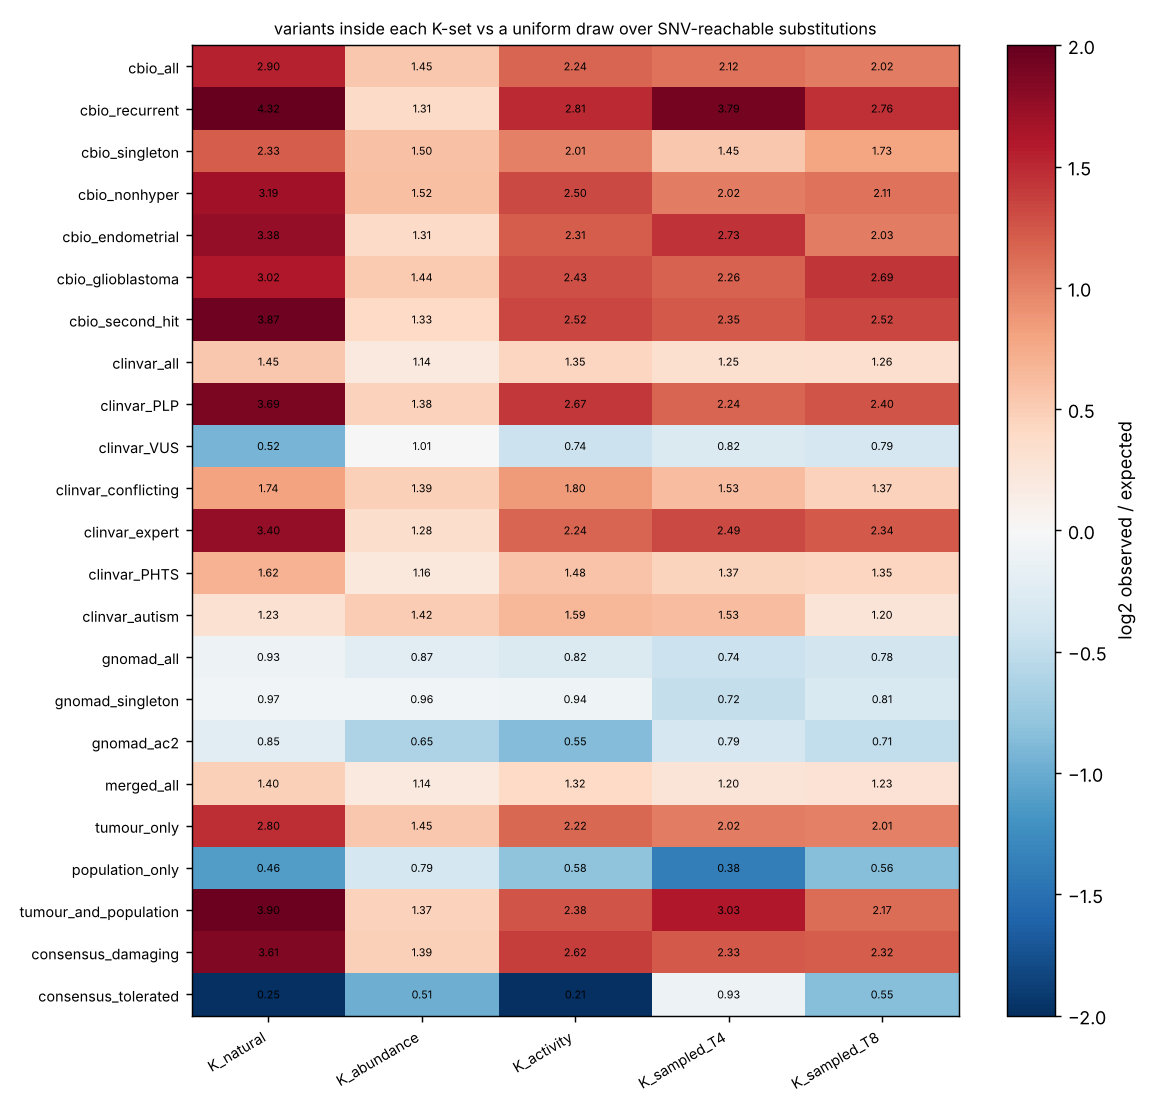
\includegraphics[width=.8\linewidth]{figures/pten_var_kset_enrichment.png}
\caption{Table~\ref{tab:enrich} as a heat map, $\log_2$(observed/expected).}
\end{figure}

\subsection{Correlations with the per-site references}

\begin{table}[H]
\centering\small
\begin{tabular}{@{}lrrrrrrrr@{}}
\toprule
 & \multicolumn{2}{c}{family entropy} & \multicolumn{2}{c}{abundance} &
 \multicolumn{2}{c}{activity} & \multicolumn{2}{c}{sampled T4} \\
Category & raw & $|$RSA & raw & $|$RSA & raw & $|$RSA & raw & $|$RSA \\
\midrule
tumour, all & $-0.46$ & $-0.36$ & $-0.30$ & $-0.11$ & $-0.56$ & $-0.47$ & $-0.35$ & $-0.22$ \\
tumour, recurrent & $-0.39$ & $-0.35$ & $-0.08$ & $+0.07$ & $-0.44$ & $-0.41$ & $-0.24$ & $-0.16$ \\
ClinVar P/LP & $-0.61$ & $-0.55$ & $-0.28$ & $-0.00$ & $-0.65$ & $-0.56$ & $-0.39$ & $-0.23$ \\
ClinVar VUS & $+0.25$ & $+0.22$ & $+0.05$ & $-0.15$ & $+0.22$ & $+0.18$ & $+0.12$ & $+0.06$ \\
gnomAD, all & $+0.13$ & $+0.10$ & $+0.14$ & $+0.10$ & $+0.06$ & $+0.01$ & $+0.06$ & $+0.01$ \\
population-only & $+0.22$ & $+0.19$ & $+0.18$ & $+0.10$ & $+0.18$ & $+0.13$ & $+0.12$ & $+0.06$ \\
consensus damaging & $\mathbf{-0.62}$ & $-0.55$ & $-0.29$ & $\mathbf{-0.02}$ & $\mathbf{-0.65}$ & $-0.56$ & $-0.40$ & $-0.25$ \\
consensus tolerated & $+0.21$ & $+0.14$ & $+0.18$ & $+0.11$ & $+0.20$ & $+0.14$ & $+0.12$ & $+0.04$ \\
\bottomrule
\end{tabular}
\caption{Spearman of the per-site density with each reference, all oriented
``higher = more tolerant'', so a negative value means the variants land where
the reference says the site cannot change. $|$RSA: burial regressed out.
$|\rho|>0.11$ is beyond chance at 5\% for $n\approx 300$ sites. $T=8$ differs
from $T=4$ by at most 0.08 (\file{kset\_density\_correlations.tsv}).}
\label{tab:corr}
\end{table}

\subsection{Profiles}

\begin{figure}[H]
\centering
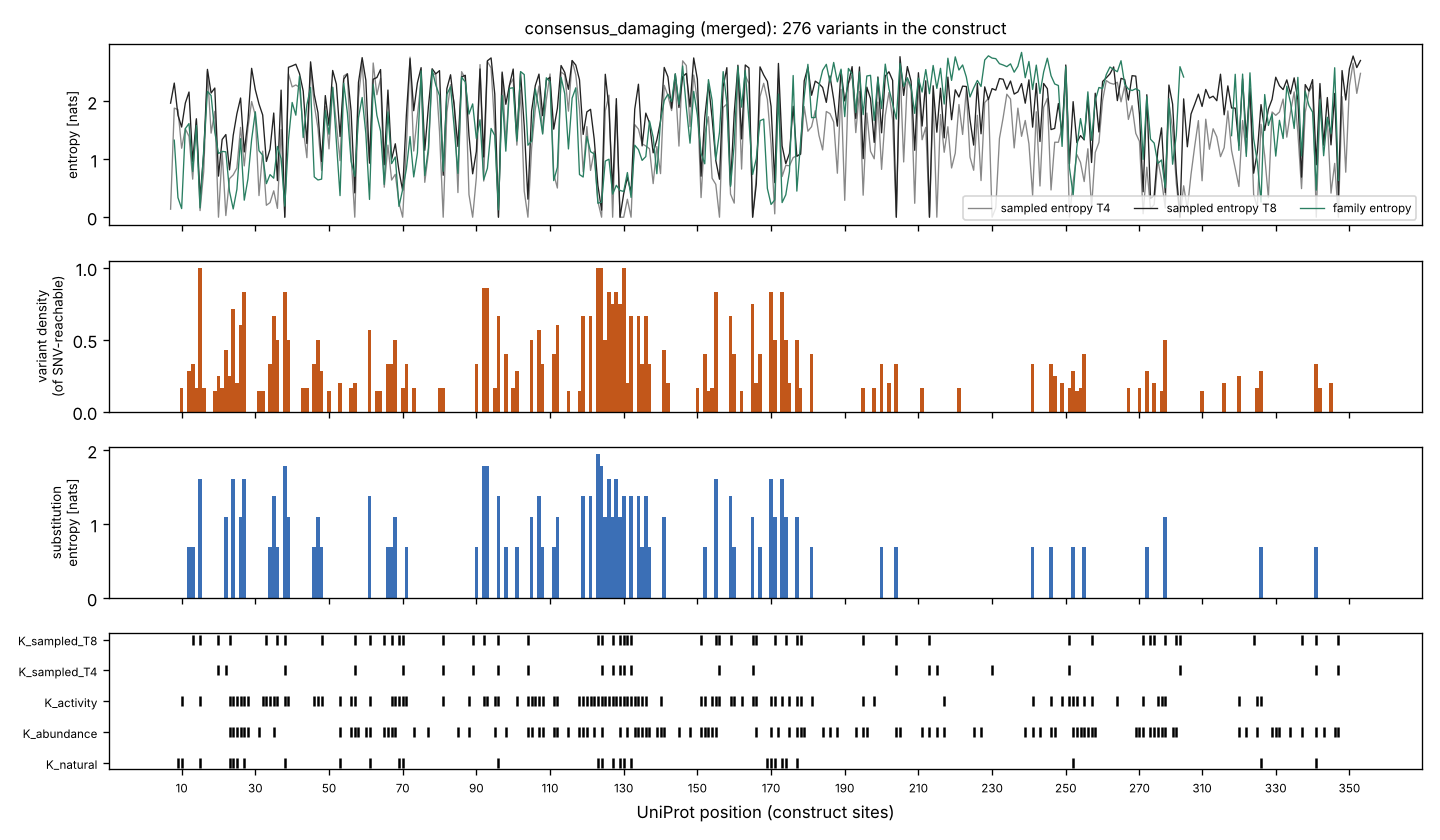
\includegraphics[width=\linewidth]{figures/pten_var_profile_consensus_damaging.png}
\caption{Consensus-damaging variants (275). From top: sampled entropy at $T=4$
and $T=8$ and the family entropy; variant density; substitution entropy; the
five K-sets. The P loop (123--130) is saturated: almost every reachable
substitution there is in the category.}
\end{figure}

\begin{figure}[H]
\centering
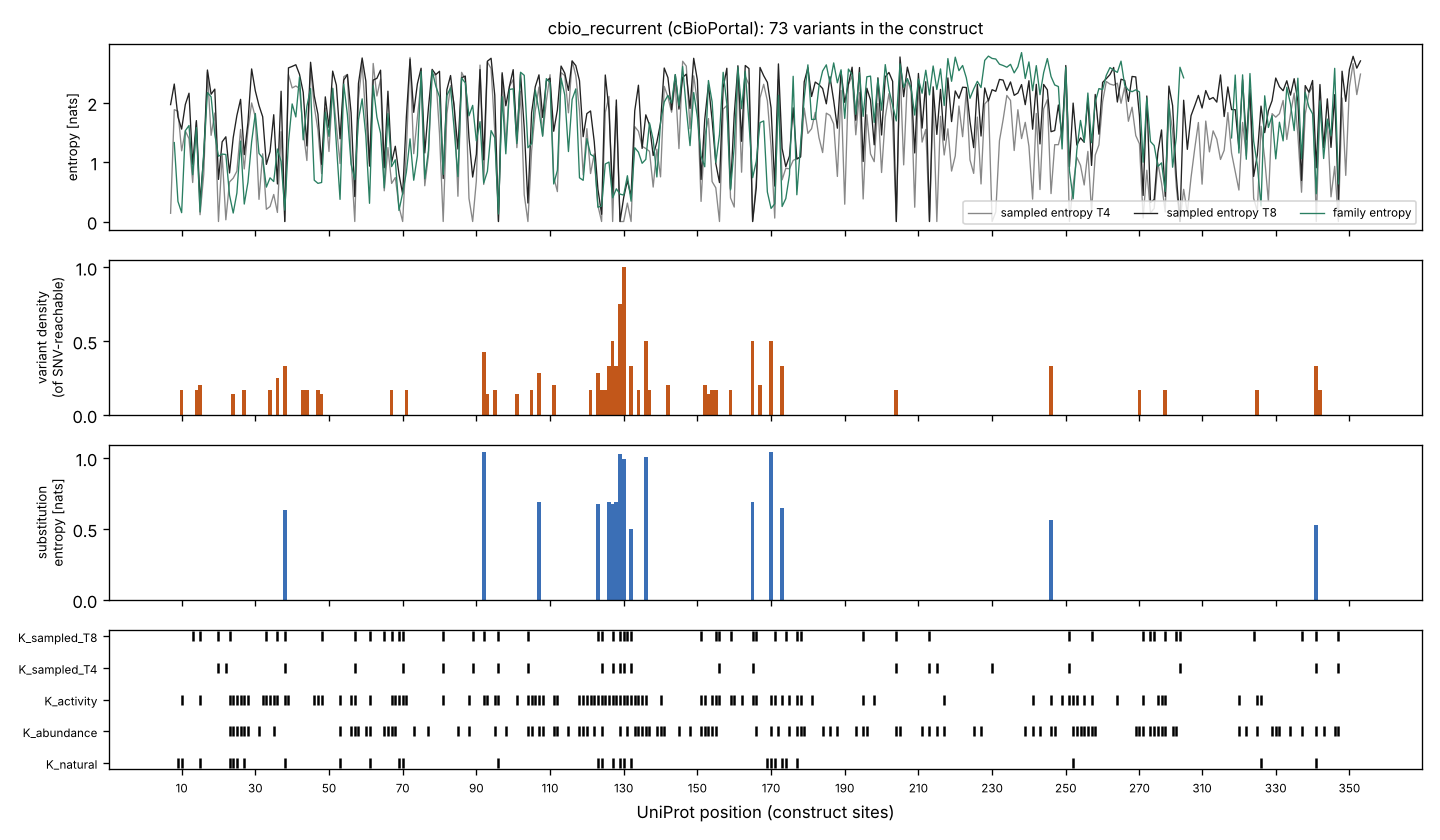
\includegraphics[width=\linewidth]{figures/pten_var_profile_cbio_recurrent.png}
\caption{Recurrent tumour variants (73, two or more patients).}
\end{figure}

\begin{figure}[H]
\centering
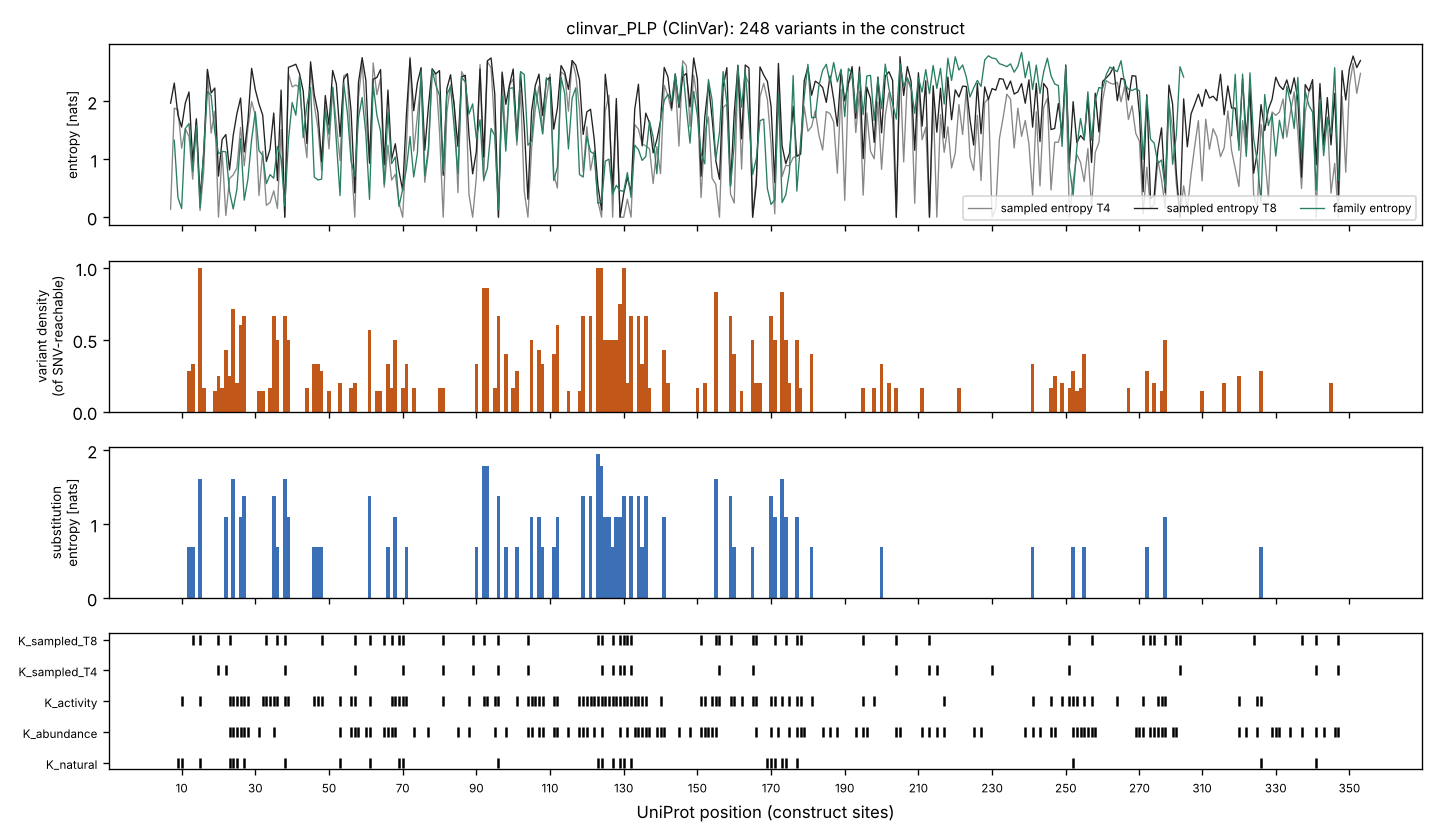
\includegraphics[width=\linewidth]{figures/pten_var_profile_clinvar_PLP.png}
\caption{ClinVar pathogenic/likely pathogenic (247).}
\end{figure}

\begin{figure}[H]
\centering
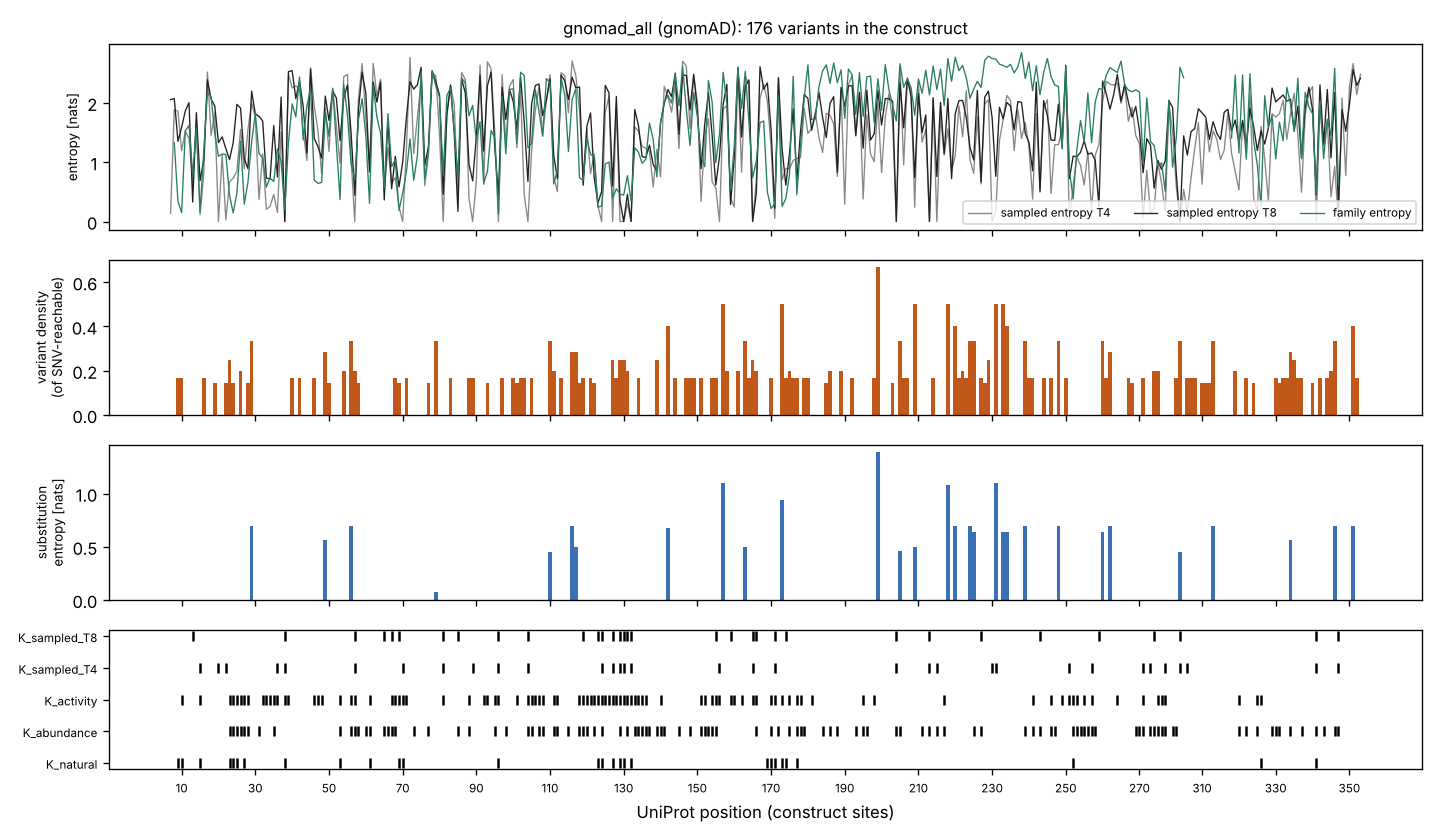
\includegraphics[width=\linewidth]{figures/pten_var_profile_gnomad_all.png}
\caption{gnomAD (176): spread along the whole construct, no relation to the
K-sets. Profiles of all 23 categories: \file{monte\_carlo/pten\_variants/kset\_profiles/}.}
\end{figure}

\subsection{What the profiles say}

\begin{enumerate}
\item \textbf{Disease variants land on conserved, catalytic sites far more
  than on fold-critical ones.} Tumour and P/LP variants are 3.6--4.3 times
  enriched in K\_natural and 2.6--2.8 times in K\_activity, against 1.3--1.4 in
  K\_abundance (table~\ref{tab:enrich}). Per site, the density of
  consensus-damaging variants follows activity ($-0.65$) and family entropy
  ($-0.62$), and both survive burial ($-0.56$, $-0.55$); its correlation with
  abundance ($-0.29$) is entirely burial ($-0.02$ given RSA). The contrast the
  K-site work found between ``conservation = catalysis'' and ``abundance =
  fold'' reappears in patients, and in patients the catalytic side is the
  one that matters.
\item \textbf{The sampler's K-sites are disease sites.} Consensus-damaging
  variants are 2.2 ($T=4$) and 2.6 ($T=8$) times enriched in them, recurrent
  tumour variants 3.2--3.3 times; the per-site density correlates $-0.40$
  with the sampled entropy, $-0.25$ after RSA. That is weaker than the family
  alignment ($-0.55$ after RSA) and clearly stronger than abundance ($-0.02$).
  The sampler's conserved core points at the sites where human disease
  mutations occur.
\item \textbf{Population variants are spread uniformly.} gnomAD sits at
  0.82--0.97 in every K-set, with no $p$ below 0.1; the stricter
  ``consensus tolerated'' class is depleted (0.25 in K\_natural, 0.21 in
  K\_activity).
\item \textbf{VUS sit where P/LP are not} (0.52 in K\_natural, positive
  correlation with tolerance). This is the classification process, not
  biology: a variant at a known critical site gets called pathogenic, and the
  uncertain ones are what remains elsewhere.
\item \textbf{Autism/macrocephaly variants are not enriched in the natural or
  sampled K-sites} (38 variants, $p\ge0.6$), only weakly in K\_activity (1.6,
  $p=0.03$). This fits the published picture of hypomorphic, partially active
  PTEN alleles in autism; with 38 variants it is a lead, not a result.
\item \textbf{The tumour signal does not depend on hypermutated samples or on
  cancer type}: non-hypermutated 3.19/2.50, endometrial 3.38/2.31,
  glioblastoma 3.02/2.43 (K\_natural / K\_activity). Variants with a
  second hit on the other allele are among the most enriched (3.87 in
  K\_natural), as expected of drivers.
\end{enumerate}

% ===========================================================================
\section{Ranking by $\Uam$, $\Etwo$ and $\Uce$}
% ===========================================================================

\subsection{Method}

Each variant inside the construct is looked up in the three scans
(\file{pten\_variants\_ranked.tsv}): its value, its percentile among all 6156
single mutants and among the 1906 SNV-reachable ones, and its rank within its
site. For each contrast between two categories, the AUC is the probability
that a variant of the first (damaging) class scores higher than one of the
second, with a 95\% bootstrap interval (1000 resamples within each class;
\file{rank.log}, \file{rank\_auc.tsv}). Alongside each energy:
\begin{itemize}
\item its \textbf{site mean} (the mean over the 19 mutants of the site), i.e.\
  what the energy knows about the site alone. The gap between the two is what
  it adds by telling substitutions apart;
\item the two experiments ($-$abundance, $-$activity, oriented the same way),
  and the \texttt{predictor\_fraction\_deleterious} column of
  \file{PTEN\_variant\_data.tsv} (the share of 15 standard predictors calling
  the variant deleterious), on the same variants;
\item AlphaMissense, available for the tumour rows only, and so reported only
  where both classes have at least 10 scored variants.
\end{itemize}
A \textbf{within-site AUC} uses only pairs of variants at the same site, one in
each class, so that burial and every other site property cancel.

\subsection{Results}

\begin{table}[H]
\centering\small
\setlength{\tabcolsep}{4pt}
\begin{tabular}{@{}R{3.9cm}ccccccc@{}}
\toprule
Contrast ($n$ pos/neg) & $\Uam$ & $\Uam$ site & $\Uce$ & $\Uce$ site & $\Etwo$ & $-$abund. & $-$activity \\
\midrule
tumour vs population-only (254/152) & 0.669 & 0.556 & 0.710 & 0.699 & 0.517 & 0.700 & 0.794 \\
 & {\scriptsize[.61,.72]} & & {\scriptsize[.66,.76]} & & {\scriptsize[.46,.57]} & & \\
tumour recurrent vs gnomAD AC$\ge$2 (73/47) & 0.698 & 0.543 & 0.770 & 0.754 & 0.486 & 0.673 & 0.855 \\
 & {\scriptsize[.60,.80]} & & {\scriptsize[.69,.85]} & & {\scriptsize[.38,.59]} & & \\
tumour non-hypermut.\ vs population-only (194/152) & 0.683 & 0.575 & 0.724 & 0.719 & 0.521 & 0.715 & 0.831 \\
ClinVar P/LP vs gnomAD not P/LP (247/152) & 0.704 & 0.548 & 0.751 & 0.721 & 0.539 & 0.768 & 0.897 \\
ClinVar P/LP vs VUS (247/624) & 0.680 & 0.554 & 0.705 & 0.659 & 0.539 & 0.678 & 0.861 \\
consensus damaging vs tolerated (275/47) & 0.698 & 0.539 & 0.762 & 0.742 & 0.495 & 0.801 & 0.901 \\
 & {\scriptsize[.60,.79]} & & {\scriptsize[.69,.84]} & & {\scriptsize[.40,.58]} & & \\
tumour recurrent vs singleton (73/181) & 0.522 & 0.484 & 0.579 & 0.541 & 0.525 & \textbf{0.386} & 0.605 \\
PHTS vs autism (665/12) & 0.507 & 0.495 & 0.502 & 0.510 & 0.572 & 0.409 & 0.559 \\
\bottomrule
\end{tabular}
\caption{AUC, higher score = damaging, SNV-reachable variants
(\file{rank.log}); 95\% bootstrap intervals in brackets for the main rows,
all of them in \file{rank\_auc.tsv}. $\Etwo$'s site mean is 0.42--0.50.
\texttt{predictor\_fraction\_deleterious}: 0.795, 0.887, 0.800, 0.847, 0.770,
0.915, 0.576, 0.373 down the rows. AlphaMissense: 0.680 (recurrent vs
singleton), 0.767 (P/LP vs gnomAD, wide interval), 0.795 (P/LP vs VUS).
On all variants, without the SNV restriction, every number moves by
$\le 0.01$, because nearly all observed variants on both sides are SNVs.}
\label{tab:auc}
\end{table}

\begin{figure}[H]
\centering
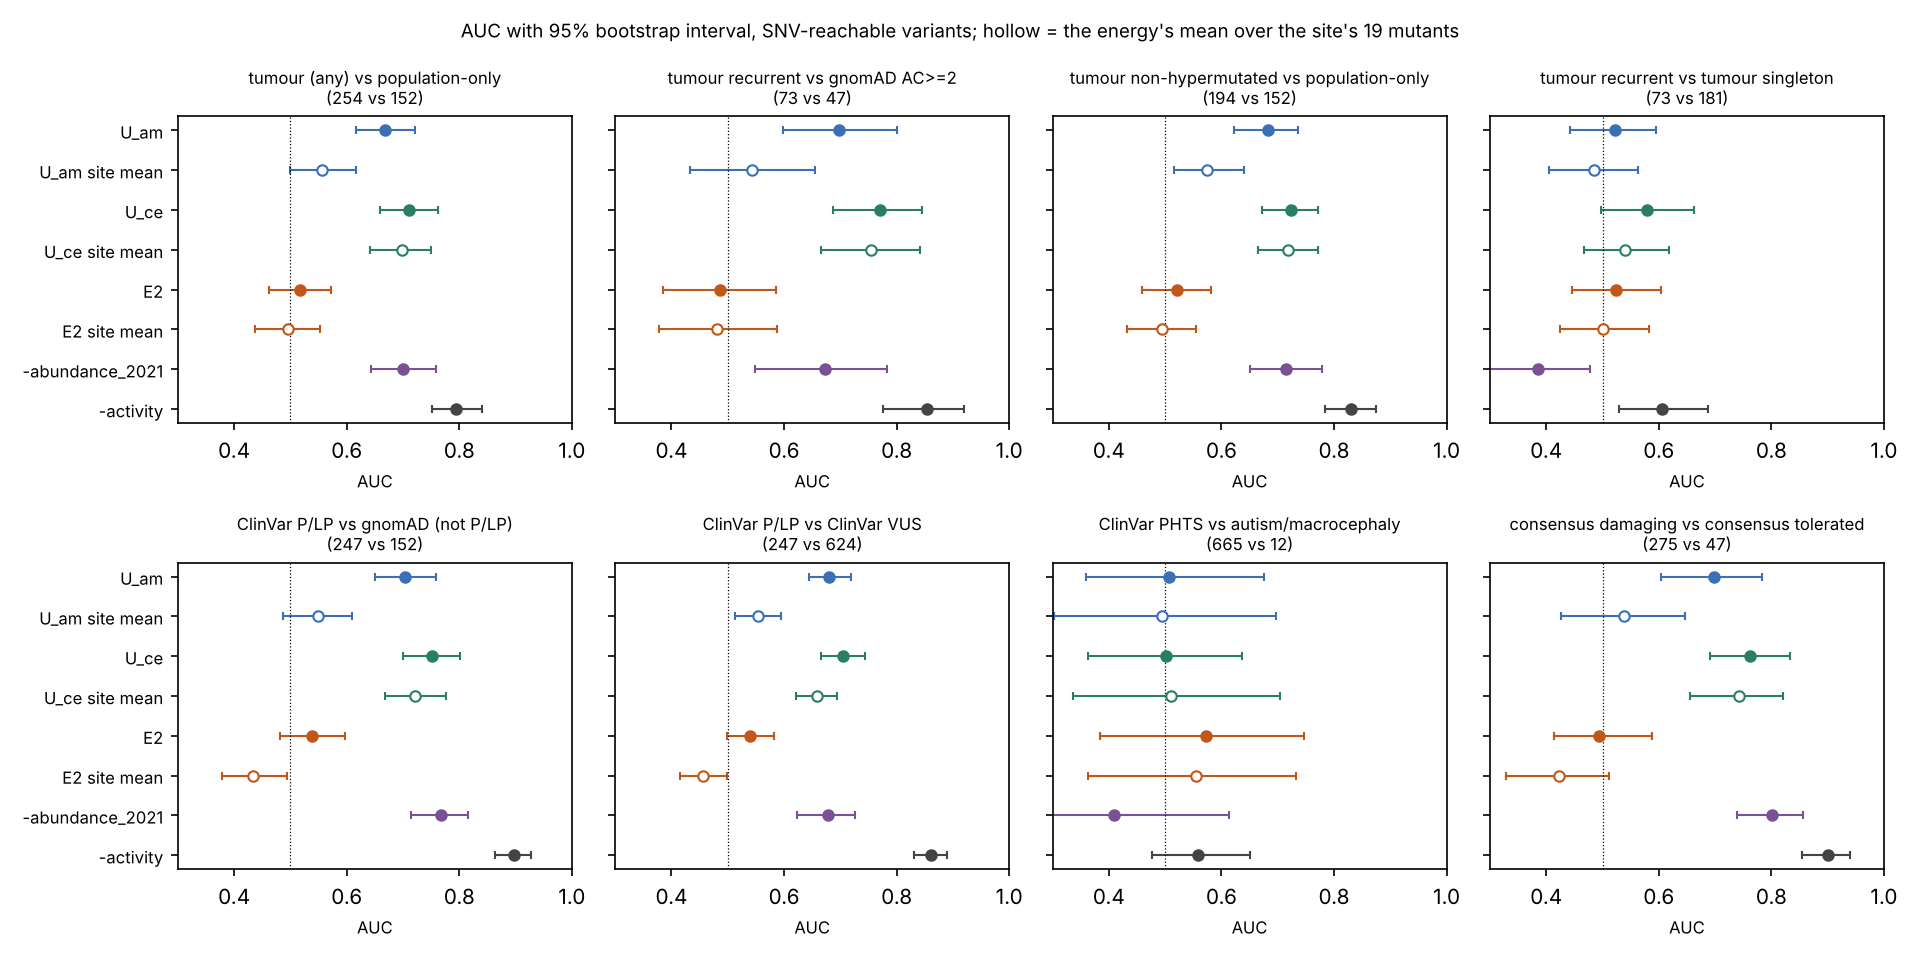
\includegraphics[width=\linewidth]{figures/pten_var_rank_auc.png}
\caption{Table~\ref{tab:auc} with intervals. Filled: the energy of the
variant itself; hollow: the energy's mean over the site's 19 mutants.}
\end{figure}

\begin{table}[H]
\centering\small
\begin{tabular}{@{}lrrrrrr@{}}
\toprule
Pairs at the same site & pairs (sites) & $\Uam$ & $\Etwo$ & $\Uce$ & $-$abund. & $-$activity \\
\midrule
ClinVar P/LP vs VUS & 232 (77) & \textbf{0.710} & 0.543 & 0.692 & 0.708 & 0.690 \\
ClinVar P/LP vs never observed & 237 (80) & 0.656 & 0.548 & 0.652 & 0.690 & 0.738 \\
tumour vs never observed & 273 (97) & 0.574 & 0.493 & 0.591 & 0.562 & 0.619 \\
tumour vs population-only & 36 (26) & 0.596 & 0.471 & 0.519 & 0.500 & 0.583 \\
population-only vs never observed & 292 (99) & 0.385 & 0.463 & 0.413 & 0.383 & 0.435 \\
\bottomrule
\end{tabular}
\caption{Within-site AUC, SNV-reachable variants. ``Never observed'' = an
SNV-reachable mutant of the scan in none of the three databases. Pair counts
are for $-$activity; the other columns differ by a few pairs.}
\label{tab:within}
\end{table}

\begin{figure}[H]
\centering
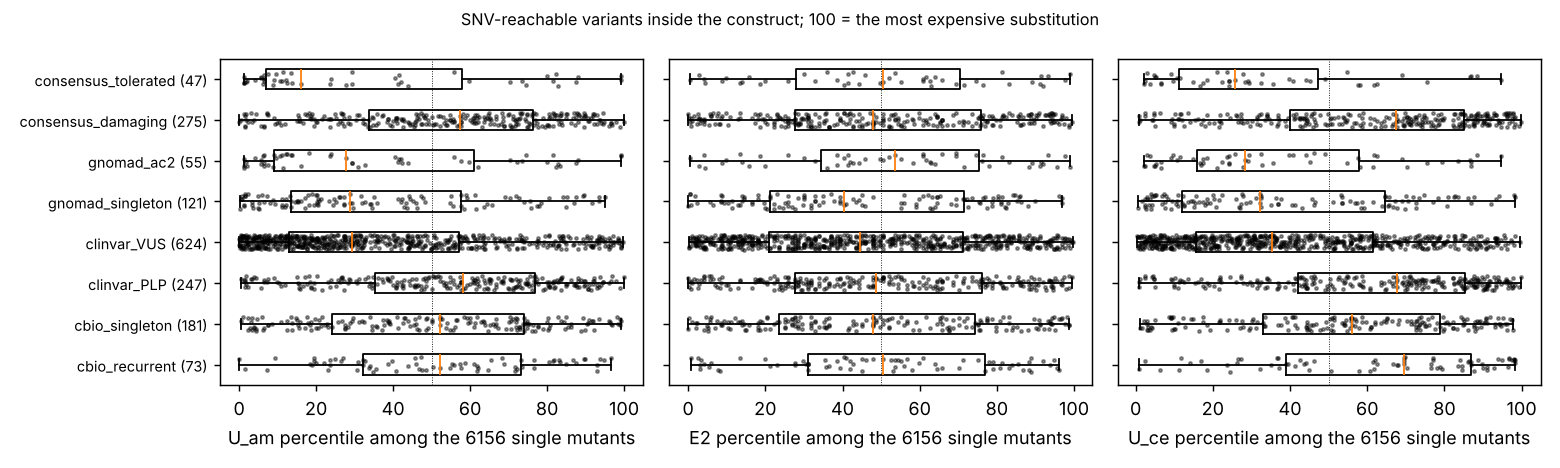
\includegraphics[width=\linewidth]{figures/pten_var_rank_by_category.png}
\caption{Percentile of each variant among the 6156 single mutants (100 = the
most expensive substitution of the construct), by category,
SNV-reachable variants. Medians in \file{rank\_percentiles.tsv}: consensus
damaging 57 ($\Uam$), 48 ($\Etwo$), 67 ($\Uce$); consensus tolerated 16, 51,
26; population-only 26, 45, 28.}
\end{figure}

\begin{table}[H]
\centering\small
\begin{tabular}{@{}lrrrrrrl@{}}
\toprule
Variant & patients & $\Uam$ pct & $\Etwo$ pct & $\Uce$ pct & abundance & activity & ClinVar \\
\midrule
R130Q & 54 & 58.6 & 59.9 & 44.0 & 1.42 & $-2.04$ & P/LP \\
R130G & 43 & 71.6 & 77.0 & 87.8 & 1.12 & $-2.14$ & P/LP \\
R173C & 13 & 83.4 & 77.9 & 86.9 & 0.16 & $-1.26$ & P/LP \\
R142W & 11 & 30.9 & 88.3 & 61.4 & 0.59 & $+0.45$ & VUS \\
G132D & 8 & 76.5 & 83.2 & 92.7 & -- & $-3.36$ & P/LP \\
C136R & 8 & 81.4 & 91.8 & 86.5 & 0.14 & $-4.79$ & P/LP \\
R130L & 7 & 80.5 & 79.0 & 86.2 & 1.20 & $-3.10$ & P/LP \\
R173H & 7 & 32.7 & 38.6 & 16.9 & 0.26 & $-1.34$ & P/LP \\
F341V & 7 & 55.8 & 93.7 & 68.1 & 0.81 & $+0.18$ & VUS \\
D92E & 6 & 23.7 & 27.7 & 67.7 & 1.06 & $-5.02$ & P/LP \\
P246L & 6 & 62.0 & 95.5 & 70.4 & 0.34 & $-1.62$ & P/LP \\
G129E & 5 & 92.9 & 8.2 & 60.8 & 0.64 & $-5.41$ & P/LP \\
R14M & 5 & 27.0 & 2.5 & 11.9 & 1.15 & $+0.45$ & -- \\
G36R & 5 & 65.4 & 3.4 & 88.6 & 0.66 & $-2.69$ & P/LP \\
\bottomrule
\end{tabular}
\caption{Tumour variants in 5+ patients: percentile among the 6156 mutants,
and the experiments (abundance 1 = wild type, 0 = nonsense-like; activity 0 =
wild type, $<-1.11$ = loss of function). ClinVar: the collapsed class; -- = not in the file.}
\label{tab:hot}
\end{table}

\begin{table}[H]
\centering\small
\begin{tabular}{@{}lrlrrrrrr@{}}
\toprule
Variant & pts & ClinVar & gnomAD AC & $\Uam$ & $\Uam$ pct & $\Uce$ pct & abundance & activity \\
\midrule
P281S & 1 & VUS & 2 & 529 & 99.1 & 88.6 & 0.91 & $+0.04$ \\
F215S & 1 & -- & 0 & 487 & 99.0 & 97.0 & 0.42 & $-1.62$ \\
M198K & 1 & P/LP & 0 & 485 & 98.9 & 84.8 & -- & $-3.97$ \\
R335P & 1 & VUS & 0 & 364 & 98.4 & 95.7 & -- & -- \\
V217G & 1 & confl. & 0 & 320 & 98.1 & 91.9 & 0.31 & $-3.08$ \\
F195S & 1 & P/LP & 0 & 232 & 96.9 & 87.6 & 0.25 & $-2.32$ \\
L325R & 2 & confl. & 0 & 220 & 96.6 & 96.7 & 0.21 & $-4.82$ \\
H272P & 1 & P/LP & 0 & 219 & 96.6 & 94.1 & 0.41 & $-3.66$ \\
G230E & 1 & VUS & 0 & 214 & 96.4 & 89.0 & 1.00 & $-0.18$ \\
F241S & 1 & P/LP & 0 & 199 & 96.0 & 66.4 & 0.21 & $-2.40$ \\
\bottomrule
\end{tabular}
\caption{The ten tumour variants with the highest $\Uam$: mostly
substitutions in the core of the C2 domain, and most of them destabilising
(abundance $\le 0.42$). P281S and G230E are the exceptions: top of the
ranking, wild-type abundance and activity.}
\label{tab:top}
\end{table}

\subsection{What the ranking says}

\begin{enumerate}
\item \textbf{$\Uam$ and $\Uce$ separate disease from population variants;
  $\Etwo$ does not.} $\Uam$ reaches 0.67--0.70 and $\Uce$ 0.70--0.77 across the
  five disease-vs-tolerated contrasts, comparable to VAMP-seq abundance
  (0.67--0.80) and below yeast activity (0.79--0.90) and the consensus of 15
  predictors (0.77--0.92). $\Etwo$ is at 0.49--0.54, and its intervals contain
  0.5 in most contrasts. This is the decisive patient-level confirmation of the
  2026-11-17 verdict on the contact-map energy.
\item \textbf{$\Uam$ ranks substitutions, $\Uce$ ranks sites} -- the same
  split found against VAMP-seq. Replacing $\Uam$ by its site mean drops it
  from 0.67--0.70 to 0.54--0.58; $\Uce$'s site mean loses at most 0.05. Within
  a site, $\Uam$ separates P/LP from VUS at 0.710, level with abundance
  (0.708) and above activity (0.690) and $\Uce$ (0.692) (table~\ref{tab:within}).
\item \textbf{Tumour hotspots are stable and catalytically dead, and fold
  energies cannot see that.} Recurrent tumour variants are \emph{more}
  abundant than singleton ones (AUC of $-$abundance 0.386): R130Q has abundance
  1.42 and activity $-2.04$, R130G 1.12 and $-2.14$, D92E 1.06 and $-5.02$
  (table~\ref{tab:hot}). Every energy is near chance on recurrent vs singleton
  (0.52--0.58), and $\Uam$ places R130Q at the 59th percentile. The commonest
  tumour mutations remove the catalytic arginine or the WPD-loop aspartate
  while leaving the fold intact. It is the patient-side form of the earlier
  scan result that $\Uam$ ``finds the pocket's packing, not its chemistry''.
\item \textbf{Being observed at all is not about cost.} Observed vs
  never-observed SNV-reachable mutants: $\Uam$ 0.516, $\Uce$ 0.562, activity
  0.633. Most observed variants are VUS and rare population alleles, which
  are as cheap as the unobserved ones. Population-only variants are
  \emph{cheaper} than unobserved mutants at their own site (within-site 0.385
  for $\Uam$), as for abundance (0.383): what survives in healthy people is
  the gentler substitution at a given position.
\item \textbf{PHTS vs autism} has 12 autism-only variants; nothing can be
  concluded.
\end{enumerate}

% ===========================================================================
\section{Compound tumour sequences}
\label{sec:compound}
% ===========================================================================

\subsection{Method}

77 tumour samples carry 2--5 PTEN missense changes; in 75, at least two fall
inside the construct (60 with two, 11 with three, 3 with four, 1 with five; 41
from hypermutated samples, 58 endometrial). Each became one sequence, the
construct with all its in-construct mutations, and \file{pten\_variants.py
score} computed its $\Uam$, $\Uce$ and $\Etwo$ on astaroth with the machinery
of the two scans: the sampler's \texttt{\_exact\_energy} at batch 1 with
$\lambda_{\mathrm{ce}}=1$ (one call gives both energies), and ESM3
\texttt{generate} at two steps, seed 0, C$_\alpha$ map at 8\,\AA. Checks in
\file{pten\_variants\_score.log}: $\Uam(\mathrm{ref}) = 0$, $\Uce(\mathrm{ref})
= 2.397402$ as in the scan. All 75 compounds took 0.2 minutes.

\paragraph{$\Etwo$ repeatability.} 50 single mutants drawn at random were
decoded again and compared with the 2-step scan run days earlier:
\textbf{50 of 50 identical} (largest difference $4.9\times10^{-7}$, Spearman
1.0000; \file{e2\_repeat.csv}). $\Etwo$ is deterministic across sessions, so
its chance-level performance above is not noise: it is what the 2-step
decode measures.

\subsection{Additivity}

\begin{table}[H]
\centering\small
\begin{tabular}{@{}lR{3.3cm}R{2.2cm}R{2.4cm}R{2.2cm}@{}}
\toprule
Energy & compound / sum of singles, median (IQR) & hypermutated / not &
Spearman, compound vs sum of singles & compound above its worst single \\
\midrule
$\Uam$ & 0.932 (0.870--0.974) & 0.925 / 0.949 & $+0.927$ & 66/75 \\
$\Uce$ & 0.773 (0.661--0.830) & 0.748 / 0.791 & $+0.894$ & 61/75 \\
$\Etwo$ & 0.492 (0.412--0.566) & 0.455 / 0.508 & $+0.495$ & 23/75 \\
\bottomrule
\end{tabular}
\caption{Compound sequences against the sum of their single mutants
(\file{rank.log}, \file{compound\_additivity.tsv}).}
\end{table}

\begin{figure}[H]
\centering
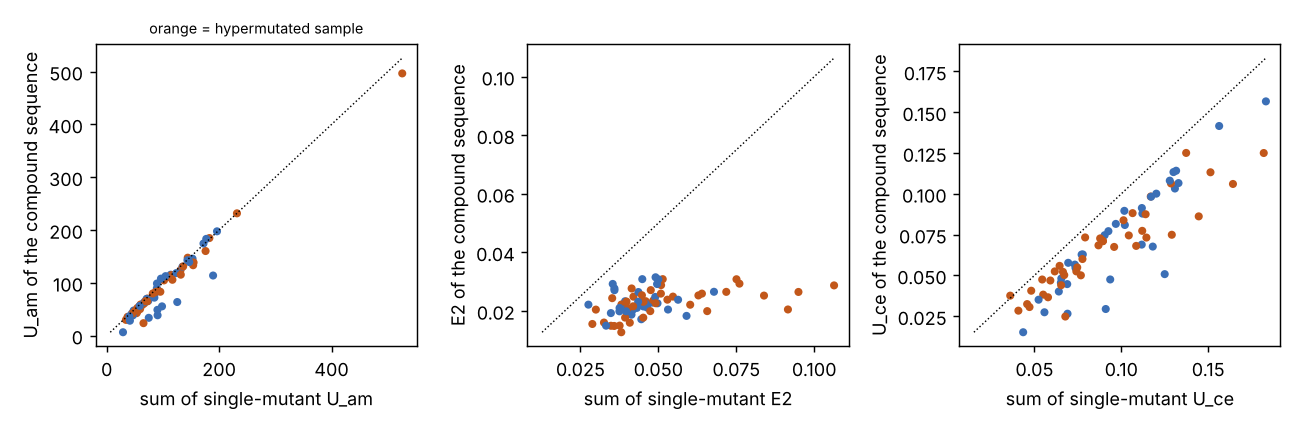
\includegraphics[width=\linewidth]{figures/pten_var_compound_additivity.png}
\caption{Each compound against the sum of its single-mutant energies;
dotted line = exact additivity; orange = hypermutated sample.}
\end{figure}

\begin{enumerate}
\item \textbf{$\Uam$ is nearly additive} (median 0.93, Spearman 0.93): two or
  three mutations scattered over PTEN cost close to the sum of their costs,
  slightly less. The extreme compound, R130Q+F215S (TCGA-BS-A0UF), costs 497
  against 526 for the sum; R130Q+P204L+R142W 232 against 232. For the sampler
  this means the landscape near the reference is close to a sum of site
  terms, the regime in which single-mutant moves are efficient.
\item \textbf{$\Uce$ is sub-additive} (0.77), still well ranked (0.89).
\item \textbf{$\Etwo$ saturates}: every compound sits at 0.013--0.031,
  whatever its singles sum to (0.49, Spearman 0.50); 52 of 75 compounds score
  no higher than their worst single. A contact-map difference at 8\,\AA\ counts
  pairs crossing the threshold, and a decode that already moves a few dozen
  contacts for one mutation moves about as many for three.
\item Hypermutated and other samples behave alike (ratios within 0.05).
\end{enumerate}

% ===========================================================================
\section{Other databases checked}
% ===========================================================================

Two further sources were exported by hand on 2026-11-19 and checked against
the merged table. Neither is in \file{databases/} and neither enters the
results above; this section records that they were looked at and what they
hold. The numbers come from one-off scripts, not from \file{pten\_variants.py}.

\subsection{MaveDB, Matreyek et al.\ 2018 VAMP-seq (urn:mavedb:00000013-a-1)}

\begin{itemize}
\item \textbf{Score.} The 2018 abundance score; Spearman 0.95 with the
  \texttt{abundance\_2021} column already used (660 shared variants).
\item \textbf{Pathogenic/benign columns of the score CSV.} Not labels: each
  calibration cuts the score at thresholds (fitted on ClinVar controls) and
  returns ACMG PS3/BS3 evidence strengths. They are the score again. The CSV's
  gnomAD and VEP columns are empty.
\item \textbf{ClinVar annotations of the variant-details file.} Genuine
  ClinVar records per candidate allele, in twelve yearly snapshots
  (02/2015 to 01/2026). On the 2026 snapshot they label 646 missense
  variants, 95\,\% identical to our ClinVar file, with 2 new. Their 115
  benign/likely-benign entries are 109 synonymous and the same 6 missense we
  already had, so there is still no benign missense class. gnomAD annotations
  are sparse (144 rows against 235 missense in our gnomAD file).
\item \textbf{What is new: label history.} Re-labelling P/LP vs VUS with the
  2018 snapshot (before functional data fed the classifications) gives
  abundance 0.69, $\Uam$ 0.66, $\Uce$ 0.67, $\Etwo$ 0.58, activity 0.70
  (69--114 per class). On the 2026 snapshot: 0.70, 0.71, 0.72, 0.51, 0.85.
  Only activity jumps, which is the circularity of Section~\ref{sec:caveats}
  made visible; the ESM3 energies do not depend on it.
\end{itemize}

\subsection{ClinGen Evidence Repository, PTEN VCEP}

\begin{itemize}
\item \textbf{Content.} Complete web exports of the PTEN Variant Curation
  Expert Panel's classifications, with the ACMG codes met: pathogenic (76),
  likely pathogenic (53), uncertain (62), likely benign (32), benign (12);
  235 distinct ClinVar records. (The first export was one 25-row page per
  class and the second had its file names shifted by one class; the
  \texttt{Classification} column was used throughout.)
\item \textbf{Missense.} 122 records: 83 P/LP (82 changes, G36R by two
  codons), 33 VUS, 6 B/LB. Every change is already in the merged table, and
  all but one carry the same class as our ClinVar file. The exception is
  M134I: the panel calls c.402G$>$C likely pathogenic and c.402G$>$A
  uncertain, which a protein-level key merges. The 6 B/LB are the same A79T,
  S229T, Q298E, S294R, P354Q, S360G (only A79T and S229T inside the
  construct), so there is still no benign missense class.
\item \textbf{Functional evidence.} 69 of 83 P/LP missense records use PS3,
  4 of 6 B/LB use BS3, and 21 of 33 VUS carry PS3 or BS3. Functional assays
  enter most expert classifications, which is the circularity again.
\item \textbf{Ranking.} P/LP vs VUS inside the construct (80 vs 27), with
  95\,\% bootstrap intervals: $\Uam$ 0.67 (0.54--0.80), $\Uce$ 0.65
  (0.53--0.77), $\Etwo$ 0.58 (0.45--0.70), abundance 0.68 (0.53--0.82; 60 vs
  19), activity 0.87 (0.79--0.95; 73 vs 25). Keeping only the 11 VUS
  classified without functional evidence: $\Uam$ 0.63, $\Uce$ 0.61, $\Etwo$
  0.60, abundance 0.69, activity 0.92. The energies sit where they sit
  against ClinVar labels, $\Etwo$'s interval contains 0.5, and activity is
  highest because it is part of the label.
\end{itemize}

Verdict: neither source changes a result. MaveDB's label history supports the
circularity caveat for the activity AUC; ClinGen's expert labels reproduce the ClinVar AUCs of the energies and show, through its evidence codes, why the activity AUC is inflated.

% ===========================================================================
\section{Caveats}\label{sec:caveats}
% ===========================================================================

\begin{itemize}
\item \textbf{Circularity on the ClinVar side.} ClinVar classifications for
  PTEN can use functional assays and computational predictors as evidence, so
  the AUCs of abundance, activity, AlphaMissense and the predictor consensus
  against ClinVar labels may be inflated. $\Uam$, $\Uce$ and $\Etwo$ never saw
  ClinVar, the experiments or the predictors.
\item \textbf{gnomAD is not benign.} It means ``seen in gnomAD'', mostly once;
  24 P/LP changes are there. The contrasts exclude P/LP from the population
  side, and the ``consensus tolerated'' class is only 47 variants.
\item \textbf{cBioPortal here is TCGA PanCancer only.} Half of the missense
  rows are endometrial; 119 of 418 samples are hypermutated. Results without
  hypermutated samples are reported and change little.
\item \textbf{One snapshot per database.} The three files were exported on
  different dates; the 19 + 1 disagreements in the cross-references are the
  visible trace of that.
\item \textbf{176 variants are outside the construct} (C-tail, the 286--309
  loop, N-terminus) and have no energy. A full-length scan would cover them
  but on a different reference, not comparable with these numbers.
\item \textbf{Only one of the 15 predictors entered.} The script picks numeric
  predictor columns from \file{PTEN\_variant\_data.tsv}; only
  \texttt{predictor\_fraction\_deleterious} qualified, as the individual calls
  are categorical. It already summarises the 15.
\end{itemize}

% ===========================================================================
\section{Summary}
% ===========================================================================

\begin{enumerate}
\item The three files hold 1269 distinct PTEN missense changes after three
  parsing traps are removed (ClinVar's shifted header, PTEN-L numbering, KLLN);
  only 22 are in all three, and gnomAD is mostly inside ClinVar.
\item Disease variants (tumour, ClinVar P/LP) concentrate on sites conserved
  in the family and required for activity, not on sites required for
  abundance; the sampler's own K-sites are enriched 2.2--3.3 times for them.
  Population variants are uniform.
\item $\Uam$ and $\Uce$ recognise disease variants at AUC 0.67--0.77, close to
  the abundance experiment; $\Uam$ does it by substitution, $\Uce$ by site. The
  two-step contact-map energy is at chance and saturates on compounds; it is
  deterministic, so that is a property of the energy, not noise.
\item The most frequent tumour mutations are stable but inactive; no energy
  that reads the fold can rank them, and that limits what an ESM3 structural
  energy can say about PTEN's tumour-suppressor function.
\item $\Uam$ is close to additive over the 2--5 mutations seen in single
  tumours.
\end{enumerate}

% ===========================================================================
\appendix
\section{Reproducing}
% ===========================================================================

From \file{softmax/monte\_carlo}:
\begin{verbatim}
python pten_variants.py clean      # traps, dedup, codons -> clean.log
python pten_variants.py merge      # overlaps, cross-refs, compounds -> merge.log
python pten_variants.py profiles   # K-sets, densities -> profiles.log
nohup python -u pten_variants.py score > pten_variants_score.log 2>&1 &   # GPU
python pten_variants.py rank       # AUCs, percentiles, compounds -> rank.log
\end{verbatim}
Options worth knowing: \texttt{--hypermutated 500}, \texttt{--temperatures T4
T8}, \texttt{--burn-in-frac 0.8}, \texttt{--sampled-k-frac 0.1},
\texttt{--min-category 20}, \texttt{--bootstrap 1000}; \texttt{score} takes
\texttt{--num-steps 2} and \texttt{--repeat 50}. Outputs in
\file{monte\_carlo/pten\_variants/}, described in its \file{README.md}.

\end{document}
